\documentclass[lang=cn,10pt,bibend=bibtex]{elegantbook}

\title{Project: 四阶有限体积方法}

\author{Wenchong Huang}
\date{Aug 20, 2023}

\setcounter{tocdepth}{3}

\logo{logo-blue.jpg}
\cover{cover.jpg}
\usepackage{multirow}
\usepackage{xpatch}
\makeatletter
\xpatchcmd{\chapter}
  {\if@openright\cleardoublepage\else\clearpage\fi}{\par\relax}
  {}{}
\makeatother

% 本文档命令
\usepackage{array, float}
\newcommand{\ccr}[1]{\makecell{{\color{#1}\rule{1cm}{1cm}}}}

% 修改标题页的橙色带
% \definecolor{customcolor}{RGB}{32,178,170}
% \colorlet{coverlinecolor}{customcolor}

\begin{document}

\maketitle
\frontmatter

\tableofcontents

\mainmatter

\chapter{用户手册}

\section{编译与测试说明}

请在项目根目录下执行以下命令完成编译:
\begin{lstlisting}
  make
\end{lstlisting}

\subsection{测试用例一、二}

对于第一个测试用例,请使用以下命令运行测试:
\begin{lstlisting}
  time ./test1 M
\end{lstlisting}

其中\verb|M|表示将区域划分为$M\times M$的网格。程序将会输出误差、求解时间,并将求解结果输出到\verb|result.txt|。在matlab中编写如下脚本即可绘制图像。
\begin{lstlisting}
  [x,y]=meshgrid(0:1/M:(1-1/M),0:1/M:(1-1/M));
  z = load("result.txt")';
  pcolor(x,y,z)
  shading interp;
\end{lstlisting}

对于第二个测试用例,运行与绘图方法与第一个测试用例完全相同,将\verb|test1|改为\verb|test2|即可。但是程序将不会输出误差,需要用matlab读取解并用Richardson外插法计算误差。

\subsection{测试用例三}

对于第三个测试用例,请使用以下命令运行测试:
\begin{lstlisting}
  time ./test3 M Re Cr eps
\end{lstlisting}

其中\verb|M|表示将区域划分为$M\times M$的网格;\verb|Re|(正整数)表示雷诺数;\verb|Cr|(正实数)表示柯朗数;\verb|eps|(正实数)表示多重网格的迭代精度。注意,\verb|eps|并不是越小越好,过小会导致求解速度很慢但解的质量几乎没有提升。

程序将会输出误差、求解时间,并将求解结果输出到\verb|result.txt|。用matlab读取时,请使用以下脚本:
\begin{lstlisting}
  sol = load("result.txt");
  ux = reshape(sol(1,:),M,M);
  uy = reshape(sol(2,:),M,M);
  p = reshape(sol(3,:),M,M);
\end{lstlisting}

\subsection{对流扩散方程求解器接口}

以测试用例一为例,求解器的调用如下。

\begin{lstlisting}
  // 新建求解器
  FV_MOL_Solver solver;
  // 设置网格大小
  solver.setGridSize(stoi(argv[1]));
  // 设置终止时间
  solver.setEndTime(1.0);
  // 设置扩散系数
  solver.setNu(nu);
  // 设置时间步长,三个参数依次为:柯朗数、ux最大值、uy最大值
  solver.setTimeStepWithCaurant(1.0, 1.0, 0.5);
  // 设置外力项
  solver.setForcingTerm(&f);
  // 设置初值条件
  solver.setInitial(&phi);
  // 设置边值条件
  solver.setBondary("down", &phi, "Dirichlet");
  solver.setBondary("left", &phi, "Dirichlet");
  solver.setBondary("up", &dyphi, "Neumann");
  solver.setBondary("right", &dxphi, "Neumann");
  // 设置速度,当速度场为常向量时,用setConstVelocity能显著提速
  solver.setConstVelocity(1.0, 0.5);
  // 求解
  solver.solve();
  // 将解输出到文件
  solver.output("result.txt");
  // 计算误差。需要提供真解、范数,在norm.h中提供了p范数、无穷范数可供调用
  cout << "Error in max-norm: " << solver.checkerr(&phi, Norm_inf()) << endl;
  cout << "Error in 1-norm: " << solver.checkerr(&phi, Norm_p(1)) << endl;
  cout << "Error in 2-norm: " << solver.checkerr(&phi, Norm_p(2)) << endl;
\end{lstlisting}

以测试用例二为例,求解器的调用如下。
\begin{lstlisting}
  FV_MOL_Solver solver;
  solver.setGridSize(stoi(argv[1]));
  solver.setEndTime(10.0);
  solver.setNu(nu);
  solver.setTimeStepWithCaurant(1.0, 0.1, 0.1);
  solver.setInitial(&initphi);
  // 设置外力项为0
  solver.setNoForcingTerm();
  // 设置边值条件为周期
  solver.setPeriodicBondary();
  // 设置速度场(非常值)
  solver.setVelocity(&ux, &uy);
  solver.solve();
  solver.output("result.txt");
\end{lstlisting}

初值条件、边值条件、外力项使用的函数均为\verb|TimeFunction2D|的派生类,其原型的一部分如下
\begin{lstlisting}
class TimeFunction2D{
public:
    virtual double at (const double &x, const double &y, const double &t) const = 0;
    virtual double intFixX(const double &x, const double &d, const double &u, const double &t) const;
    virtual double intFixY(const double &y, const double &d, const double &u, const double &t) const;
    virtual double int2D(const double &l, const double &r, const double &d, const double &u, const double &t) const;
    virtual double accInt2D(const double &l, const double &r, const double &d, const double &u, const double &t) const;
    virtual double int2D_order6(const double &l, const double &r, const double &d, const double &u, const double &t) const;
    virtual double accInt2D_order6(const double &l, const double &r, const double &d, const double &u, const double &t) const;
};
\end{lstlisting}

用户的自定义函数必须继承\verb|TimeFunction2D|,并实现函数\verb|at(x,y,t)|,其返回值为用户自定义函数在$(x,y,t)$处的点值。若用户知道函数积分的解析表达式,也可以在子类中覆盖\verb|intFixX|(固定$x$对$y$积分)和\verb|intFixY|(固定$y$对$x$积分)。此外,若用户知道二重积分的解析表达式,建议用户将\verb|int2D|、\verb|accInt2D|、\verb|int2D_order6|、\verb|accInt2D_order6|全部覆盖。例如,测试用例二的$u_x$应该定义为:
\begin{lstlisting}
  class FUNCUX : public TimeFunction2D{
    public:
        double at (const double &x, const double &y, const double &t) const{
            return 0.1 * sin(pi*x) * sin(pi*x) * sin(2*pi*y);
        }
        double intFixX(const double &x, const double &d, const double &u, const double &t) const{
            return 0.1 * sin(pi*x) * sin(pi*x) * (cos(2*pi*d) - cos(2*pi*u)) / (2*pi);
        }
        double intFixY(const double &y, const double &d, const double &u, const double &t) const{
            return 0.1 * sin(2*pi*y) * (2*pi*(u-d) + sin(2*pi*d) - sin(2*pi*u)) / (4*pi);
        }
    } ux;
\end{lstlisting}

\subsection{INSE求解器接口}

INSE求解器的调用与对流扩散方程求解器类似。以测试用例三为例,INSE求解器的调用如下,我们在不同之处添加了注释。
\begin{lstlisting}
  INSE_Solver solver;
  solver.setGridSize(stoi(argv[1]));
  solver.setEndTime(0.5);
  solver.setNu(nu);
  solver.setTimeStepWithCaurant(stod(argv[3]), 3.0, 3.0);
  solver.setNoForcingTerm();
  // 设置初值(u为包含两个元素的TimeFunction2D指针数组)
  solver.setInitial(u);
  // 设置多重网格的迭代精度,若不设,则默认为1e-9
  solver.setEps(stod(argv[4]));
  solver.solve();
  solver.output("result.txt");
  // 计算误差,需要提供速度场真解(包含两个元素的TimeFunction2D指针数组)、压强真解(TimeFunction2D指针)、范数。checkerr的返回值为一个数组,包含3个元素,分别为ux、uy、p的数值解误差
  auto err = solver.checkerr(u, p, Norm_inf());
  cout << "Error in max-norm:\t" << err[0] << "\t" << err[1] << "\t" << err[2] << endl;
\end{lstlisting}

注意,我们的求解器只支持周期边界条件,因此不提供设置边界条件的接口。

\newpage

\chapter{数值积分}

\section{辛普森法则}

本文中的辛普森法则均指辛普森1/3法则,它是Newton-Cotes公式在$n=2$时的情形。辛普森法则用于估计如下形式的一维闭区间积分:
\begin{equation*}
  \int_a^b f(x) \;\text{d}x.
\end{equation*}

其估计如下:
\begin{equation*}
  I^S(f;a,b) = \frac{b-a}{6}\left(f(a)+4f\left(\frac{a+b}{2}\right)+f(b)\right).
\end{equation*}

对于辛普森法则的误差估计,我们有:
\begin{equation*}
  \left|I^S(f;a,b)-\int_a^b f(x) \;\text{d}x\right|\leq \frac{(b-a)^5}{2880}M,
\end{equation*}

其中$M$为$|f^{(4)}(x)|$的最大值。

\section{Boole法则}

Boole法则是Newton-Cotes公式在$n=4$时的情形。Boole法则对一维闭区间积分估计如下:
\begin{equation*}
  I^B(f;a,b) = \frac{b-a}{90}\left(7f(a)+32f\left(\frac{3a+b}{4}\right)+12f\left(\frac{a+b}{2}\right)+32f\left(\frac{a+3b}{4}\right)+7f(b)\right).
\end{equation*}

对于Boole法则的误差估计,我们有:
\begin{equation*}
  \left|I^B(f;a,b)-\int_a^b f(x) \;\text{d}x\right|\leq \frac{(b-a)^7}{945\times 2^{11}}M,
\end{equation*}

其中$M$为$|f^{(6)}(x)|$的最大值。

\section{二重积分}

对于二重积分
\begin{equation*}
  \int_a^b\int_c^d f(x,y) \;\text{d}y\;\text{d}x,
\end{equation*}

可以应用一维闭区间积分公式两次,得到对应的二重积分公式。例如,应用辛普森法则,我们有:
\begin{align*}
  I^{S,2D}(f;a,b,c,d)&= \left[\left(f(a,c)+4f\left(\frac{a+b}{2},c\right)+f(b,c)\right)\right.\\
  &+ 4\left(f\left(a,\frac{c+d}{2}\right)+4f\left(\frac{a+b}{2},\frac{c+d}{2}\right)+f\left(b,\frac{c+d}{2}\right)\right)\\
  &+ \left.\left(f(a,d)+4f\left(\frac{a+b}{2},d\right)+f(b,d)\right)\right] \times \frac{(b-a)(d-c)}{36}
\end{align*}

而误差估计可以为
\begin{equation*}
  \left|I^{S,2D}(f;a,b,c,d)-\int_a^b\int_c^d f(x,y) \;\text{d}y\;\text{d}x\right| = O((b-a)^5),
\end{equation*}

或
\begin{equation*}
  \left|I^{S,2D}(f;a,b,c,d)-\int_a^b\int_c^d f(x,y) \;\text{d}y\;\text{d}x\right| = O((d-c)^5),
\end{equation*}

对于Boole法则,有类似的结果。

\section{自适应积分}

我们希望把积分计算得更加精确,最好将误差控制在预先给定的$\varepsilon$以内。例如,在二维区域中,用某种法则计算积分值,记为$A$;然后将区域四等分,用同样的法则分别计算4个等分区域的积分值,记作$A_1,...,A_4$,然后计算误差:
\begin{equation*}
  E=|A-\sum_{i=1}^4 A_i|.
\end{equation*}

若$E<\varepsilon$,则将$\sum_{i=1}^4 A_i$作为结果返回,否则递归计算四个子区域。

\section{应用场景}

计算初值、真解的积分值时,我们将使用用自适应积分方法,将误差控制在$10^{-14}$以内。

考虑到在求解过程中计算面积分、体积分时应用自适应方法代价过大,因此求解过程中,遇到要算积分,我们将直接使用积分公式。对于一维平均积分,使用辛普森法则,有误差估计:
\begin{equation*}
  \frac{1}{h}\int_i^{i+h} g(x) \;\text{d}x=\frac{1}{h}I^S(g;i,i+h)+O(h^4).
\end{equation*}

对于二维平均积分,辛普森公式的阶数不够,因此采用Boole法则导出的二重积分公式,有误差估计:
\begin{equation*}
  \frac{1}{h^2}\int_i^{i+h}\int_j^{j+h} f(x,y) \;\text{d}y\;\text{d}x=\frac{1}{h^2}I^{B,2D}(f;i,i+h,j,j+h)+O(h^5).
\end{equation*}

\vspace{6em}

\chapter{代数多重网格}

为节省工作量,本文所有求解器的解方程部分均采用代数多重网格。经测试,选取恰当的强依赖阈值,可以使代数多重网格的性能与几何多重网格相当,甚至超越几何多重网格\footnote{这项比较基于我的结果(代数多重网格)、樊睿的结果(几何多重网格)、凌子恒的结果(几何多重网格)。}。本章的内容来源于我在微分方程数值解课程中的多重网格大作业,并额外添加了3.6节。

\section{背景与介绍}

代数多重网格(AMG)是几何多重网格的一个自然推广,当我们发现由偏微分方程引出的离散方程组,使用多重网格具有如此优秀的表现时,自然会想,能不能将其推广到更一般的方程组,解更一般的大型稀疏矩阵。

答案是肯定的,这就是代数多重网格。具体而言,代数多重网格对$M$矩阵具有较好的表现,$M$矩阵是满足正定对称、对角元为正数、非对角元非正的矩阵。事实上,大部分椭圆方程的离散矩阵都是$M$矩阵。

对一个$n\times n$的矩阵$A^h$,我们不妨将$1,...,n$看作点,将$A^h$看作一个邻接矩阵,这样我们就得到了一个稀疏图,于是就有了网格结构。

要想应用多重网格的思路,我们必须将方程限制到粗网格中,求解后返回细网格调整。但此时我们面临着严峻的问题:我们不知道网格的结构,只知道一个矩阵。我们需要一些算法来选取粗网格点$\Omega^{2h}$,并且定义限制算子$I_{h}^{2h}$与插值算子$I_{2h}^{h}$,还要给出粗网格上的矩阵$A^{2h}$。

\section{选取粗网格点}

要想从中选取粗网格点,首先给出如下定义:

\begin{definition}
  若$i,j$满足:
  \begin{equation}
    |a_{i,j}|\geq \theta\max_{k\neq i}|a_{i,k}|
  \end{equation}

  则称$i$强依赖于$j$,也称$j$强影响$i$. 其中$\theta$是一个事先给定的阈值,称为“强依赖阈值”.

  记$N_i$为所有使$a_{i,j}\neq 0$的点$j$构成的集合,称为“相邻点”集。记$S_i$为所有强影响$i$的点构成的集合,$S_i^T$为所有强依赖于$i$的点构成的集合。
\end{definition}

在下文中,我们记粗网格$\Omega^{2h}=C$,细网格$\Omega^h=C\cup F$,即$F$表示所有在细网格但不在粗网格中的点。我们还记$C_i=S_i\cap C,\;D_i^s=S_i\cap F,\;D_i^w=N_i\setminus S_i$.

我们希望用一种\textbf{启发式的方法}来选取粗网格点,具体地,我们希望:
\begin{enumerate}[(1)]
  \item $\forall i\in F$,对于$j\in S_i$,或$j\in C_i$,或$j$强依赖于$C_i$中某点;
  \item $C$中的点尽可能多,但需要保持:$\forall i\in C$,没有$j\in C$使得$i$强依赖于$j$。
\end{enumerate}

当然,我们只是希望上述性质尽可能得到满足,为此,William L. Briggs的书上给出了\textbf{“染色算法”},如下:
\begin{enumerate}[1]
  \item $C,F\gets \varnothing$, $\lambda_i\gets |S_i^T|$.
  \item 选取$i\in\Omega^h\setminus(C\cup F)$,使$\lambda_i$最大.
  \item $C\gets C\cup\{i\}$, $F\gets F\cup (S_i^T\setminus C)$.
  \item $\forall j\in S_i^T,\;\forall k\in S_j\setminus(C\cup F)$, 令$\lambda_k\gets \lambda_k+1$.
  \item 若$C\cup F=\Omega^h$,结束,否则返回第2步.
\end{enumerate}

注意到上述过程需要维护一个$\lambda_i$数组,支持增加、删除、求最大下标三种操作,我们期望单次操作的复杂度不超过$O(\log n)$,因此我们实现了一个\textbf{二叉搜索树}。当然,使用线段树、平衡树也是可以的,不过因为可以提前建树,所以平衡操作是不必要的。

\section{构建插值算子}

对于$\mathbf{e}\in\Omega^{2h}$,插值算子具有如下格式:
\begin{equation}
  (I_{2h}^h \mathbf{e})_i=\left\{
    \begin{array}{ll}
      e_i & \text{若 }i\in C,\\
      \sum_{j\in C_i}\omega_{ij}e_j & \text{若 }i\in F.
    \end{array}
  \right.
\end{equation}

在粗网格中,我们求解的方程是$A^{2h}\mathbf{e}=\mathbf{f}$,其中$\mathbf{f}$是光滑化(即若干次G-S迭代)后的残差,通常比较小,因此
\begin{equation*}
  a_{ii}e_i\approx -\sum_{j\in N_i} a_{ij}e_j.
\end{equation*}

将$N_i$展开成三类,得
\begin{equation}
  a_{ii}e_i\approx -\sum_{j\in C_i} a_{ij}e_j -\sum_{j\in D^s_i} a_{ij}e_j -\sum_{j\in D^w_i} a_{ij}e_j.
\end{equation}

对于$j\in D^w_i$,将$e_j$近似为$e_i$,得
\begin{equation}
  \left(a_{ii}+\sum_{j\in D^w_i} a_{ij}\right)e_i\approx -\sum_{j\in C_i} a_{ij}e_j -\sum_{j\in D^s_i} a_{ij}e_j.
\end{equation}

对于$e_j\in D_i^s$,将其近似为
\begin{equation}
  e_j\approx \frac{\sum_{k\in C_i} a_{jk}e_k}{\sum_{k\in C_i} a_{jk}}.
\end{equation}

将(6.5)代入(6.4),得
\begin{equation}
  \omega_{ij}=-\frac{a_{ij}+\sum\limits_{m\in D_i^s}\left(\frac{a_{im}a_{mj}}{\sum\limits_{k\in C_i} a_{mk}}\right)}{a_{ii}+\sum\limits_{n\in D_i^w} a_{in}}
\end{equation}

本小节内容均来源于William L. Briggs的书,我们实现了上述过程,同时对反复使用的求和进行了预处理优化,能在$O(N_i)$的时间里完成单个$\omega_{ij}$的计算。

\section{构建限制算子与粗网格矩阵$A^{2h}$}

事实上,有了插值算子,我们可以直接由对称性和Garlerkin条件构建$I_{h}^{2h}$与$A^{2h}$,如下:
\begin{equation}
  I_{h}^{2h}:=(I_{2h}^{h})^T
\end{equation}
\begin{equation}
  A^{2h}:=I_{h}^{2h}A^hI_{2h}^{h}
\end{equation}

\section{V-Cycle}

实际上,代数多重网格的V-Cycle与几何多重网格基本一致,只不过使用的$A^h,I_h^{2h},I_{2h}^h$都是事先构建好的。为方便表述,记\verb|Rh|为$I_{h}^{2h}$,\verb|Ph|为$I_{2h}^{h}$,下面以递归形式描述。

\begin{lstlisting}
    VC(h, x, f)
        if size of grid <= 16
            return direct_solve(Ah, f)
        pre-smoothing for v1 times
        e = VC(2h, zeros, Rh*(f-Ah*x))
        x = x + Ph * e
        post-smoothing for v2 times
        return x
\end{lstlisting}

有了V-Cycle,自然可以定义FMG-Cycle.

\section{纯Neumann条件或周期条件下的求解}

对于纯Neumann条件或周期条件下的二维Poisson方程,我们知道,在解存在的前提下,任何两个解都相差一个常数。此时直接使用多重网格求解也是可以的,但是解会发生“漂移”,即平均值越来越大。这对数值方法很不友好,实际测试时,一个$512\times 512$的二维网格所需的FMG迭代次数可以高达$30$次。为此,我们人为添加“平均值为$0$”的额外条件,并定义下面这个操作为\textbf{“均值标准化”}。

\begin{equation*}
  \mathbf{v}\gets \mathbf{v}-\left(\frac{1}{n}\sum_{i=1}^n v_i\right)\mathbf{e}.
\end{equation*}

我们在第一层网格中,每进行完一次smoothing都对当前解执行一次均值标准化,实测效果极佳,可以将FMG迭代次数降低到5次以内。这个做法可以在文献\cite{Multigrid}的第113页找到。

\textbf{在INSE的近似投影算子中,我们将会用到本节的做法}。

\newpage

\chapter{对流扩散方程的四阶MOL方法}

\section{设计要点}

求解器均按讲义上的四阶公式按部就班实现。特别地,当$u_d$为常向量时,$L_{\text{adv}}$可直接由(12.38)与(12.9)得到;否则$L_{\text{adv}}$需要由(12.38)、(12.24)、(12.25)与(12.9)得到。

另外,每当遇到ghost cell时,就用(12.29)、(12.30)代入。

\subsection{优化之一:网格预生成}

注意到步骤(12.40b)中需要求解一个方程组,而这个方程组的系数矩阵是不变的,因此只需要一个AMG求解器,在程序的一开始完成初始化、网格生成,这将节省大量时间。

\subsection{优化之二:保存中间结果}

注意到$\mathbf{X}^{[E]}(\phi^{(j)},t^{(j)})$、$\mathbf{X}^{[I]}(\phi^{(j)})$要用到$(7-j)$次,为了避免重复计算,将计算结果保存。这样每个RK步原本$\mathbf{X}^{[E]}$与$\mathbf{X}^{[I]}$各需计算21次,经优化后只需计算6次。

\section{测试用例一}

该测试用例的真解为
\begin{equation*}
  \phi(x,y,t)=\sin(2\pi x-t)\sin(4\pi y-0.5t).
\end{equation*}

扩散系数$\nu=0.01$,由对流扩散方程可以导出外力项。下面左图为初值,右图为$t=1$时刻的真解。

\begin{figure}[H]
  \centering
  \begin{minipage}[t]{0.49\linewidth}
      \centering
      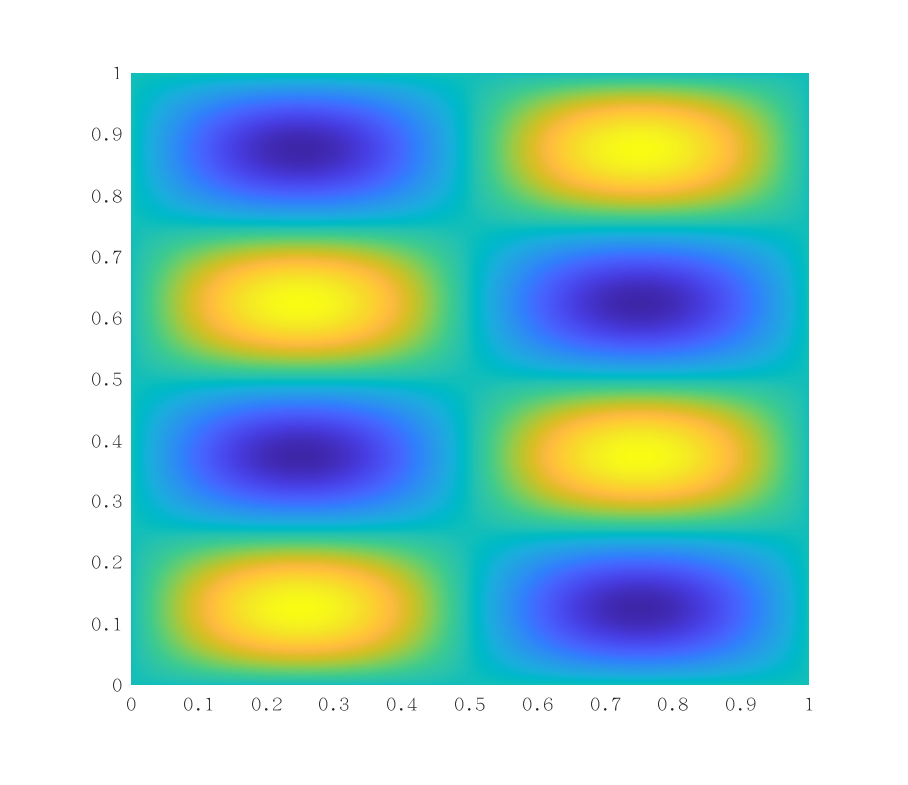
\includegraphics[width=0.9\linewidth]{figure/test1_init.eps}
      \caption*{$t=0$时的初值}
  \end{minipage}
  \begin{minipage}[t]{0.49\linewidth}
    \centering
    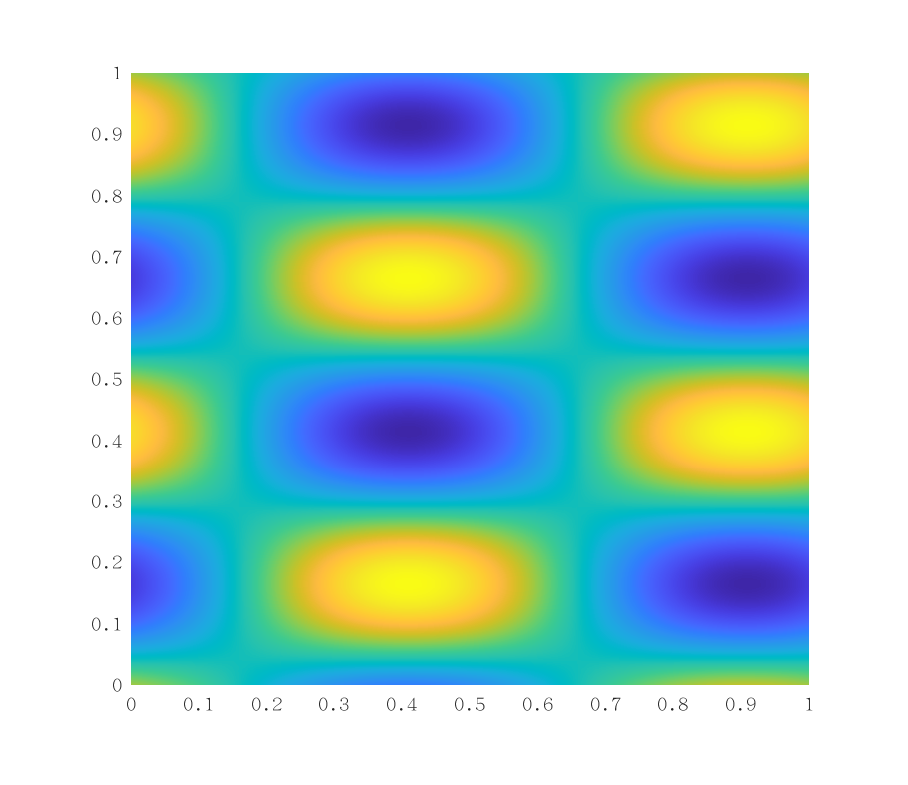
\includegraphics[width=0.9\linewidth]{figure/test1_end.eps}
    \caption*{$t=1$时的真解}
  \end{minipage}
\end{figure}

在右边界、上边界用Neumann边值条件,在左边界、下边界用Dirichlet边值条件。测试结果如下

\begin{table}[H]
  \centering
  \small
  \begin{tabular}{c|ccccccc}
  \textbf{$M$}              & 64          & 收敛阶 & 128         & 收敛阶 & 256         & 收敛阶 & 512   \\ \hline
  1范数误差                  & 2.17966e-05 & 3.96  & 1.39805e-06 & 3.98  & 8.88880e-08 & 3.98  & 5.63568e-09 \\
  2范数误差                  & 2.83356e-05 & 3.97  & 1.80426e-06 & 3.98  & 1.14017e-07 & 3.99  & 7.19684e-09 \\
  $\infty$范数误差           & 8.12398e-05 & 4.00  & 5.08051e-06 & 4.00  & 3.16646e-07 & 4.00  & 1.97709e-08 \\
  运行时间(s)                & 5           &       & 52          &       & 622         &       & 5694
  \end{tabular}
\end{table}

下面是$M=64$和$M=128$的误差分布图。可以看到,若忽略尺度,二者误差分布基本一致。靠近Dirichlet条件的边界误差较小,靠近Neumann条件边界误差较大。

\begin{figure}[H]
  \centering
  \begin{minipage}[t]{0.49\linewidth}
      \centering
      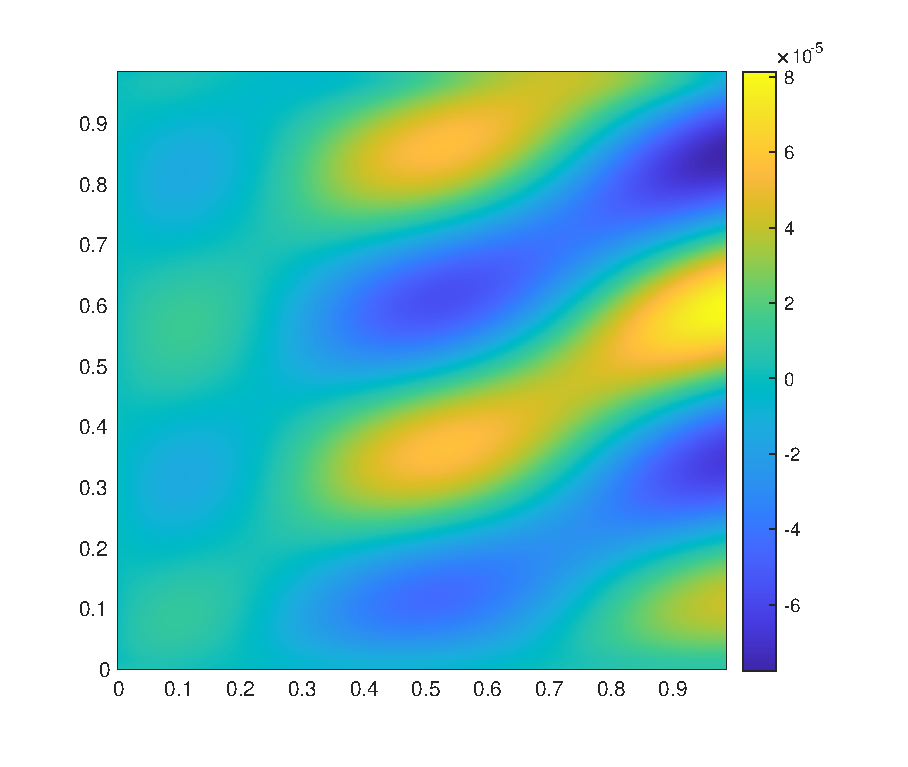
\includegraphics[width=0.9\linewidth]{figure/test1_error64.eps}
      \caption*{$M=64$的误差分布图}
  \end{minipage}
  \begin{minipage}[t]{0.49\linewidth}
    \centering
    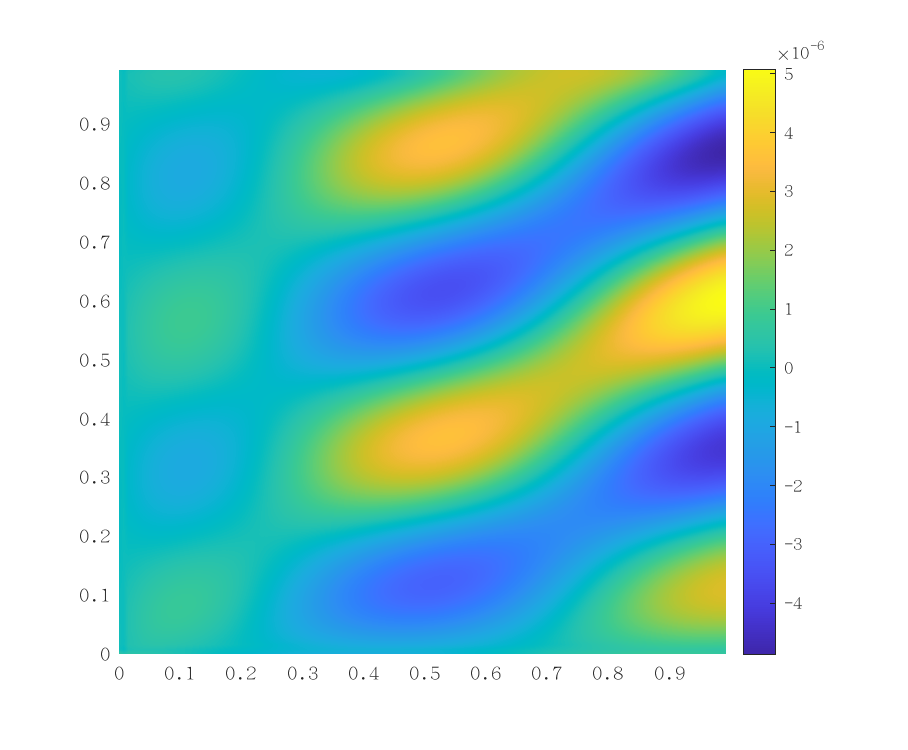
\includegraphics[width=0.9\linewidth]{figure/test1_error128.eps}
      \caption*{$M=128$的误差分布图}
  \end{minipage}
\end{figure}

\section{测试用例二}

该用例的初值由下面的函数给出。
\begin{equation*}
  \phi(x,y) = \exp\left(\frac{(x-c_x)^2+(y-c_y)^2}{0.01/\ln 10^{-16}}\right).
\end{equation*}

其中$(c_x,c_y)=(0.5,0.75)$。另外,扩散系数$\nu=0.001$,速度场为
\begin{equation*}
  \mathbf{u}(x,y) = 0.1(\sin^2(\pi x)\sin(2\pi y), -\sin(2\pi x)\sin^2(\pi y)).
\end{equation*}

可以计算积分的解析表达式:
\begin{equation*}
  \int_a^b u_1(x,y) \;\text{d}x= \frac{\sin(2\pi y)}{40\pi}(2\pi(b-a)+\sin(2\pi a)-\sin(2\pi b)),
\end{equation*}
\begin{equation*}
  \int_a^b u_1(x,y) \;\text{d}y= \frac{\sin^2(\pi x)}{20\pi}(\cos(2\pi a)-\cos(2\pi b)),
\end{equation*}

对$u_2$也有类似结果。

从初始时刻$t_0=0$开始,演化至终止时刻$t_e=10$。下面左图为初值,右图为$512\times 512$网格的仿真结果。

\begin{figure}[H]
  \centering
  \begin{minipage}[t]{0.49\linewidth}
      \centering
      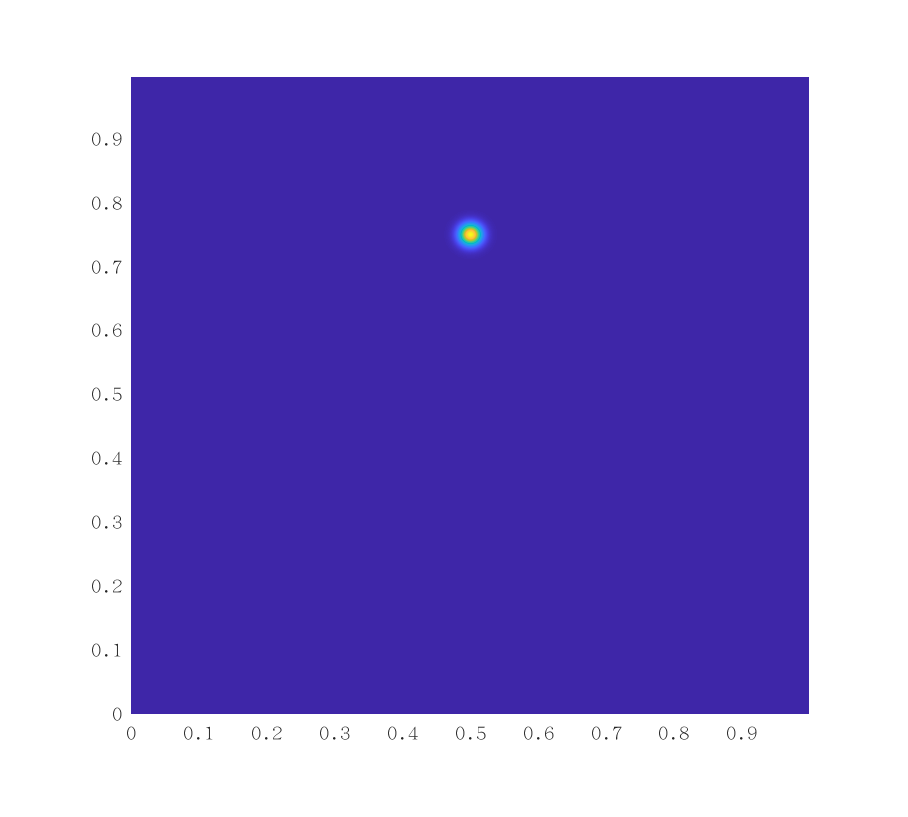
\includegraphics[width=0.9\linewidth]{figure/test2_init.eps}
      \caption*{$t=0$时的初值}
  \end{minipage}
  \begin{minipage}[t]{0.49\linewidth}
    \centering
    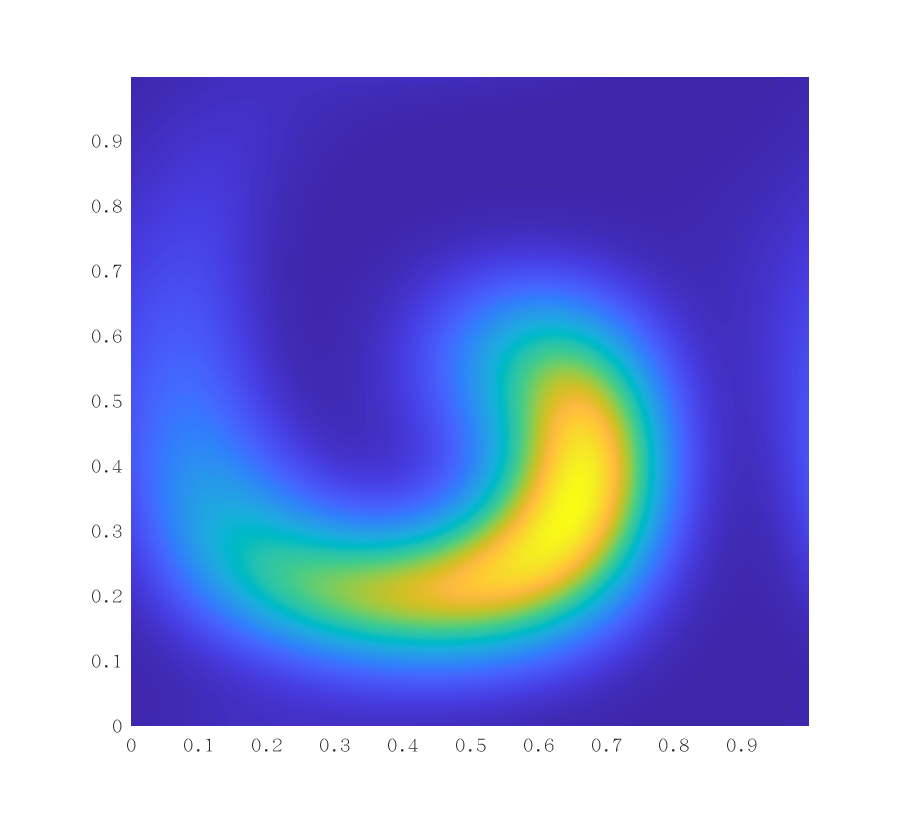
\includegraphics[width=0.9\linewidth]{figure/test2_end.eps}
    \caption*{$512\times 512$的网格在$t=10$时刻的计算结果}
  \end{minipage}
\end{figure}

由于真解未知,我们采用Richardson外插法来估计误差与收敛阶。具体而言,以$2M\times 2M$网格上的解作为真解计算$M\times M$网格的求解误差,记作$E(M)$,那么收敛阶可以由$\log_2\frac{E(M)}{E(2M)}$计算得到。这个做法见LeVeque书\cite{2007Finite}上的第257页。

我们在$M=64,128,256,512$的网格上依次求解,当然,为了使用上述方法估计误差,还需要$M=1024$的结果,我们也一并计算。结果如下。

\begin{table}[H]
  \centering
  \small
  \begin{tabular}{c|ccccccc}
  \textbf{$M$}              & 64          & 收敛阶 & 128         & 收敛阶 & 256         & 收敛阶 & 512   \\ \hline
  1范数误差                  & 9.74830e-08 & 3.98  & 6.18924e-09 & 3.99  & 3.88379e-10 &  4.00 & 2.42993e-11 \\
  2范数误差                  & 1.75527e-07 & 3.98  & 1.11599e-08 & 3.99  & 7.00492e-10 &  4.00 & 4.38596e-11 \\
  $\infty$范数误差           & 7.90676e-07 & 3.94  & 5.16717e-08 & 3.99  & 3.26315e-09 &  3.99 & 2.05022e-10 \\
  运行时间(s)                & 5           &       & 41          &       & 390         &       & 3503
  \end{tabular}
\end{table}

下面是$M=64$和$M=128$的误差分布图。可以看到,若忽略尺度,二者误差分布基本一致。

\begin{figure}[H]
  \centering
  \begin{minipage}[t]{0.49\linewidth}
      \centering
      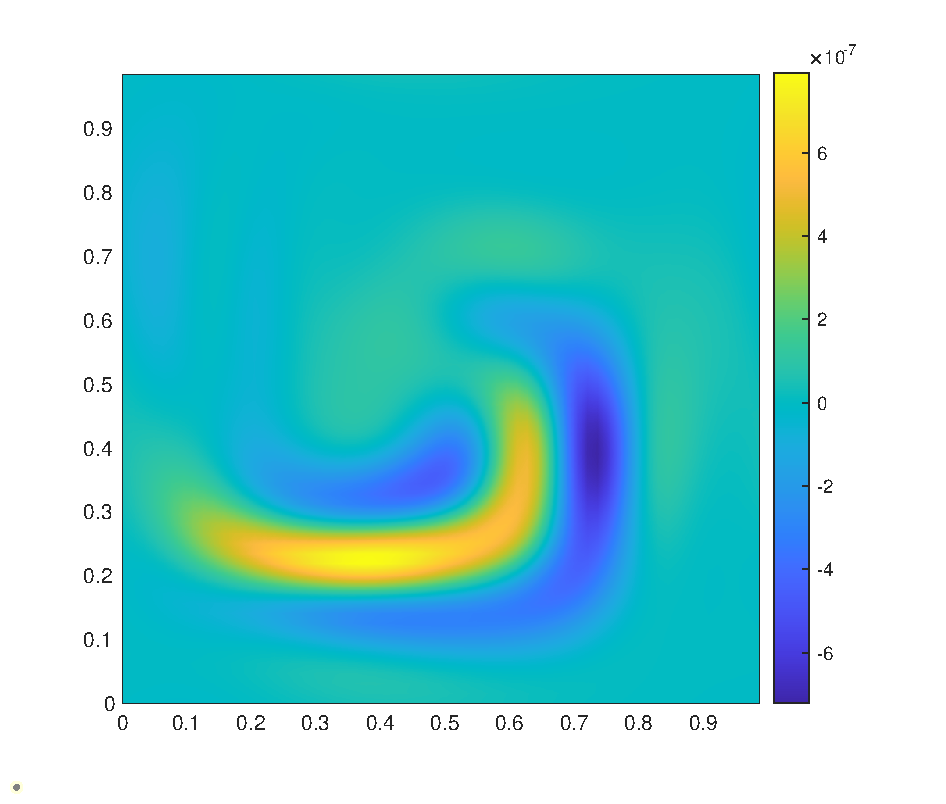
\includegraphics[width=0.9\linewidth]{figure/test2_error64.eps}
      \caption*{$M=64$的误差分布图}
  \end{minipage}
  \begin{minipage}[t]{0.49\linewidth}
    \centering
    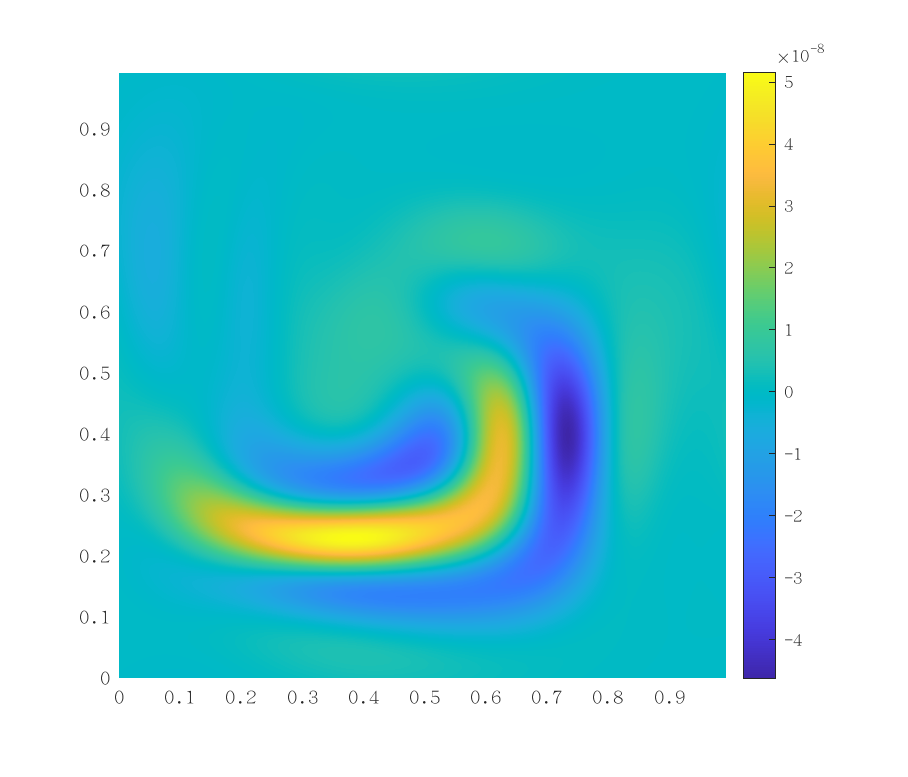
\includegraphics[width=0.9\linewidth]{figure/test2_error128.eps}
      \caption*{$M=128$的误差分布图}
  \end{minipage}
\end{figure}

\vspace{4em}

\chapter{INSE的四阶近似投影方法}

\section{设计要点}

大致与对流扩散方程求解器是类似的,按讲义上的公式实现。最主要的区别在于INSE的求解需要用到近似投影算子
\begin{equation*}
  \mathbf{P}=\mathbf{I}-\mathbf{GL}^{-1}\mathbf{D}.
\end{equation*}

从表达式上可以看出,需要解一个Poisson方程。由于我们默认使用周期边界,这个Poisson方程的解仅在相差一个常数意义下唯一(求解方法见3.6节),但我们会对解用$\mathbf{G}$算子作用一次,从而消除相差一个常数的影响,使得算子$\mathbf{P}$的作用确实具有唯一结果。

\subsection{优化之一:网格预生成}

我们由两个地方需要求解方程,一个是近似投影算子中的$\mathbf{L}^{-1}$,另一个是隐RK方法要求解的方程。这两个方程的系数矩阵是不会变的,因此我们只需要两个AMG求解器,并在一开始将每层网格预生成好,在之后的求解过程中就可以直接迭代,节省大量时间。

\subsection{优化之二:保存中间结果}

为避免重复计算,我们需要保存的中间结果有:$\mathbf{L}\langle\mathbf{u}\rangle^{(j)}$、$\mathbf{X}^{[E]}\langle\mathbf{u}\rangle^{(j)}$、$\mathbf{PX}^{[E]}\langle\mathbf{u}\rangle^{(j)}$。另外注意,$\mathbf{PX}^{[E]}\langle\mathbf{u}\rangle^{(s)}$是用不到的,因此无需计算。
\vspace{-1em}

\section{测试用例三}

该测试用例采用周期边值条件,真解为
\begin{equation*}
  \mathbf{u}(x,y,t)=1+2\exp(-8\pi^2\nu t)\left(\begin{array}{c}
    -\cos(2\pi(x-t))\sin(2\pi(y-t))\\
    \sin(2\pi(x-t))\cos(2\pi(y-t))
  \end{array}\right),
\end{equation*}
\begin{equation*}
  p(x,y,t)=-\exp(-16\pi^2\nu t)(\cos(4\pi(x-t))+\cos(4\pi(y-t))).
\end{equation*}

代入INSE,可以求得外力项为0。我们考虑雷诺数为$Re=30,300,3000,30000$,终止时刻设为$t_e=0.5$,流速场的解如下图所示。

\vspace{-1em}
\begin{figure}[H]
  \centering
  \begin{minipage}[c]{0.49\linewidth}
      \centering
      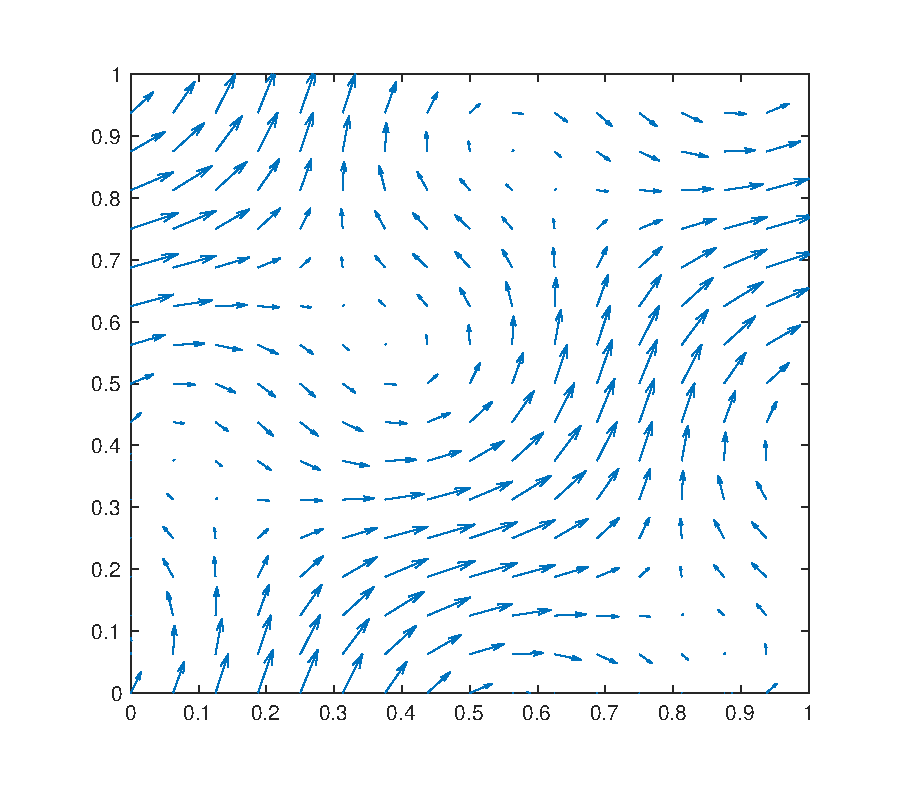
\includegraphics[width=0.9\linewidth]{figure/test3_init.eps}
      \caption*{初始时刻的流速场}
  \end{minipage}
  \begin{minipage}[c]{0.49\linewidth}
    \begin{minipage}[t]{0.49\linewidth}
      \centering
      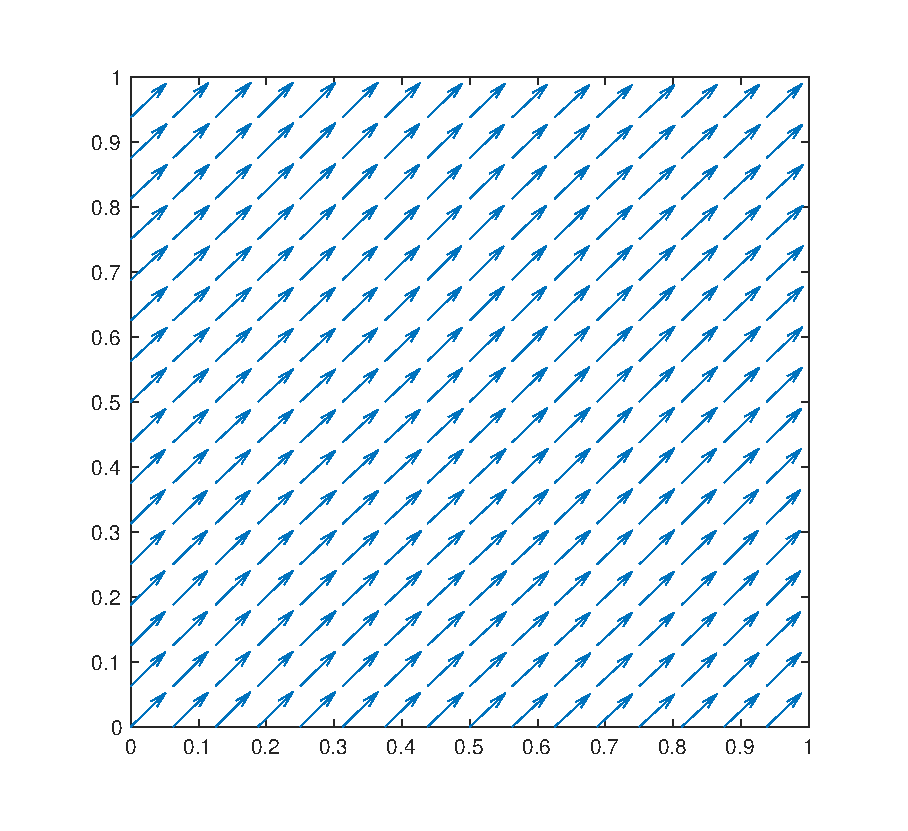
\includegraphics[width=0.95\linewidth]{figure/test3_Re=30.eps}
      \caption*{$Re=30$的解}
      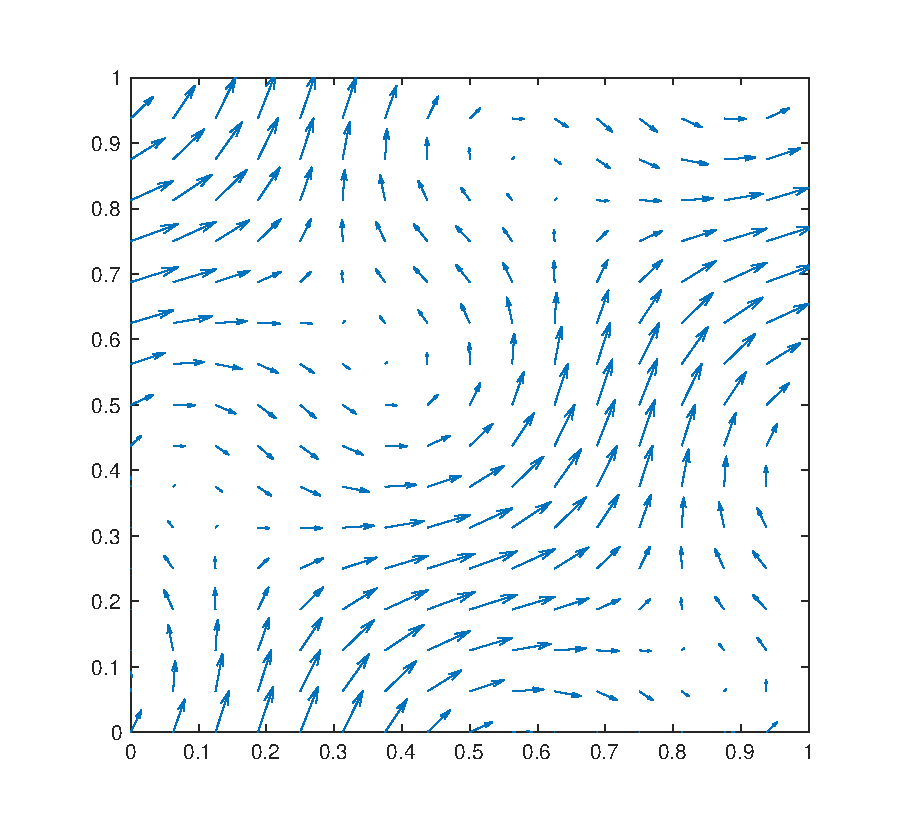
\includegraphics[width=0.95\linewidth]{figure/test3_Re=3000.eps}
      \caption*{$Re=3000$的解}
    \end{minipage}
    \begin{minipage}[t]{0.49\linewidth}
      \centering
      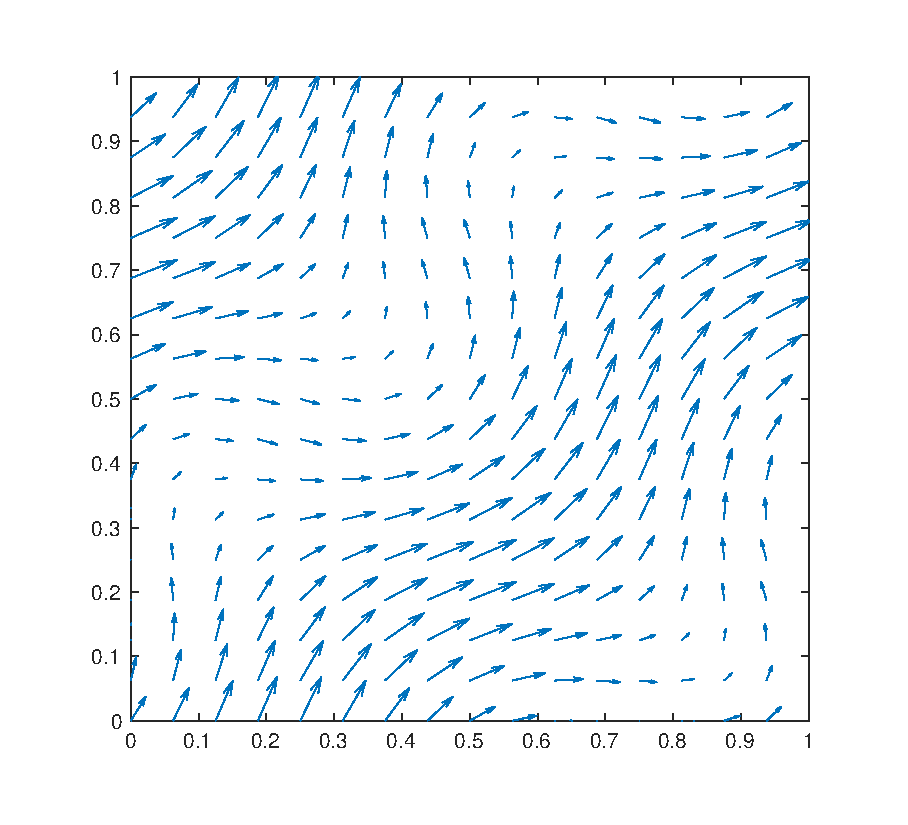
\includegraphics[width=0.95\linewidth]{figure/test3_Re=300.eps}
      \caption*{$Re=300$的解}
      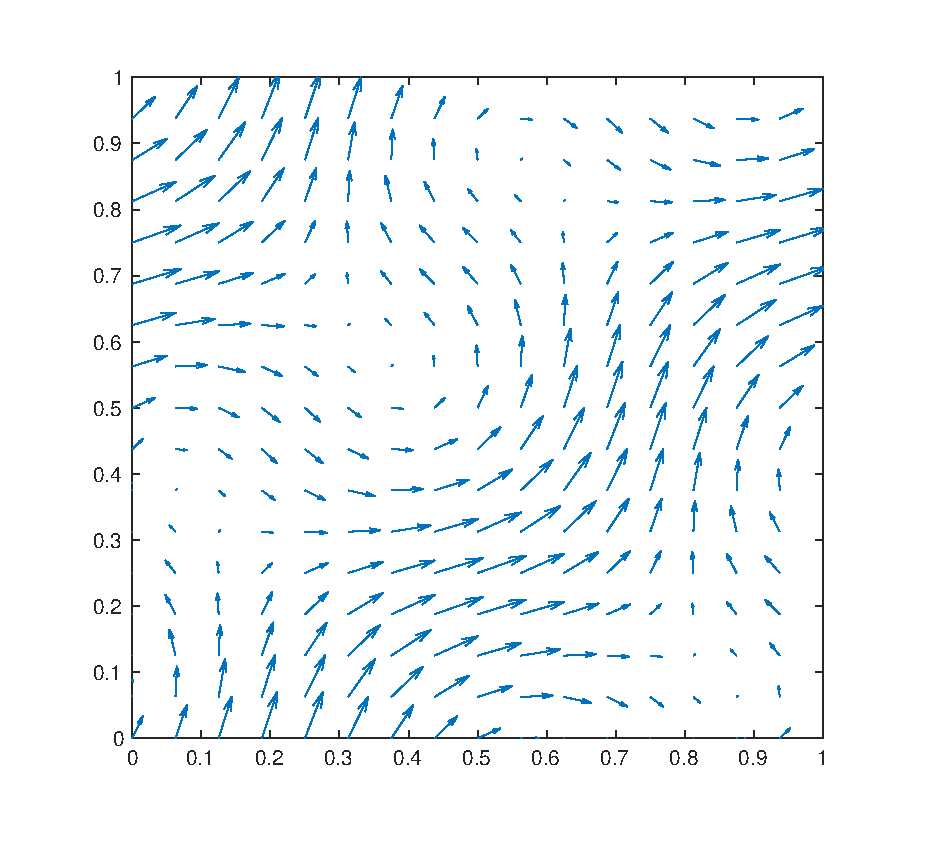
\includegraphics[width=0.95\linewidth]{figure/test3_Re=30000.eps}
      \caption*{$Re=30000$的解}
    \end{minipage}
\end{minipage}
\end{figure}
\vspace{-1em}

可以看到,雷诺数较小时,流速场迅速扩散,最终趋近于一个常量场;雷诺数较大时,流速场几乎不扩散。我们在$M=64,128,256,512$的网格上测试,并测试不同的柯朗数,结果如下。

\subsection{$Re=30,Cr=1.5$}
\vspace{-1em}
\begin{table}[H]
  \centering
  \small
  \begin{tabular}{c|ccccccc}
  \textbf{$M$}              & 64          & 收敛阶 & 128         & 收敛阶 & 256         & 收敛阶 & 512   \\ \hline
  $u_x$的1范数误差 & 2.19276e-07 & 3.91 & 1.46208e-08 & 3.95 & 9.43702e-10 & 3.98 & 5.99314e-11\\
  $u_x$的2范数误差 & 2.44155e-07 & 3.9 & 1.63318e-08 & 3.95 & 1.0563e-09 & 3.98 & 6.71548e-11\\
  $u_x$的$\infty$范数误差 & 3.78744e-07 & 3.85 & 2.6335e-08 & 3.93 & 1.73373e-09 & 3.96 & 1.11113e-10\\
  $u_y$的1范数误差 & 2.19275e-07 & 3.91 & 1.46208e-08 & 3.95 & 9.43702e-10 & 3.98 & 5.99315e-11\\
  $u_y$的2范数误差 & 2.44155e-07 & 3.90 & 1.63318e-08 & 3.95 & 1.0563e-09 & 3.98 & 6.71548e-11\\
  $u_y$的$\infty$范数误差 & 3.78743e-07 & 3.85 & 2.63352e-08 & 3.93 & 1.73374e-09 & 3.96 & 1.11117e-10\\
  $p$的1范数误差 & 1.34598e-08 & 4.10 & 7.86135e-10 & 4.04 & 4.76839e-11 & 4.00 & 2.98489e-12\\
  $p$的2范数误差 & 1.6603e-08 & 4.10 & 9.69736e-10 & 4.04 & 5.89009e-11 & 3.95 & 3.8051e-12\\
  $p$的$\infty$范数误差 & 3.3125e-08 & 4.09 & 1.93908e-09 & 3.60 & 1.60427e-10 & 1.80 & 4.5953e-11\\  
  运行时间(s)                &      38      &       &     280      &       &     2439     &       &  18563
  \end{tabular}
\end{table}

可以看到,速度场保持了四阶,压强的$\infty$范数出现掉阶现象,时间增长符合预期。

\subsection{$Re=30,Cr=0.75$}

\begin{table}[H]
  \centering
  \small
  \begin{tabular}{c|ccccccc}
  \textbf{$M$}              & 64          & 收敛阶 & 128         & 收敛阶 & 256         & 收敛阶 & 512   \\ \hline
  $u_x$的1范数误差 & 2.31118e-07 & 3.95 & 1.49372e-08 & 3.98 & 9.49103e-10 & 3.99 & 5.98036e-11\\
  $u_x$的2范数误差 & 2.58209e-07 & 3.95 & 1.67217e-08 & 3.97 & 1.06367e-09 & 3.99 & 6.70608e-11\\
  $u_x$的$\infty$范数误差 & 4.16974e-07 & 3.92 & 2.74776e-08 & 3.96 & 1.76218e-09 & 3.98 & 1.11547e-10\\
  $u_y$的1范数误差 & 2.31118e-07 & 3.95 & 1.49372e-08 & 3.98 & 9.49103e-10 & 3.99 & 5.98036e-11\\
  $u_y$的2范数误差 & 2.58209e-07 & 3.95 & 1.67217e-08 & 3.97 & 1.06367e-09 & 3.99 & 6.70608e-11\\
  $u_y$的$\infty$范数误差 & 4.16976e-07 & 3.92 & 2.74776e-08 & 3.96 & 1.76219e-09 & 3.98 & 1.11548e-10\\
  $p$的1范数误差 & 1.24656e-08 & 4.04 & 7.59097e-10 & 4.02 & 4.68377e-11 & 4.00 & 2.91763e-12\\
  $p$的2范数误差 & 1.53765e-08 & 4.04 & 9.36601e-10 & 4.02 & 5.78018e-11 & 3.99 & 3.63429e-12\\
  $p$的$\infty$范数误差 & 3.07007e-08 & 4.03 & 1.87322e-09 & 3.97 & 1.19422e-10 & 2.22 & 2.57001e-11\\  
  运行时间(s)                &     51       &       &    552       &       &     4817     &       &  33525
  \end{tabular}
\end{table}

可以看到,速度场保持了四阶,压强的$\infty$范数出现掉阶现象,时间增长符合预期。

\subsection{$Re=300,Cr=1.5$}

\begin{table}[H]
  \centering
  \small
  \begin{tabular}{c|ccccccc}
  \textbf{$M$}              & 64          & 收敛阶 & 128         & 收敛阶 & 256         & 收敛阶 & 512   \\ \hline
  $u_x$的1范数误差 & 1.37513e-05 & 5.05 & 4.14963e-07 & 4.25 & 2.17731e-08 & 3.72 & 1.65223e-09\\
  $u_x$的2范数误差 &  1.63715e-05 & 5.04 & 4.98193e-07 & 4.24 & 2.64294e-08 & 3.82 & 1.87062e-09\\
  $u_x$的$\infty$范数误差 & 4.36466e-05 & 5.11 & 1.26424e-06 & 4.36 & 6.16438e-08 & 4.17 & 3.4344e-09\\
  $u_y$的1范数误差 & 1.37513e-05 & 5.05 & 4.14963e-07 & 4.25 & 2.17731e-08 & 3.72 & 1.65223e-09\\
  $u_y$的2范数误差 & 1.63715e-05 & 5.04 & 4.98193e-07 & 4.24 & 2.64294e-08 & 3.82 & 1.87062e-09\\
  $u_y$的$\infty$范数误差 & 4.36466e-05 & 5.11 & 1.26423e-06 & 4.36 & 6.16436e-08 & 4.17 & 3.43443e-09\\
  $p$的1范数误差 & 3.17448e-05 & 4.48 & 1.41843e-06 & 4.25 & 7.45809e-08 & 4.10 & 4.33552e-09\\
  $p$的2范数误差 & 3.86435e-05 & 4.48 & 1.73405e-06 & 4.24 & 9.16544e-08 & 4.10 & 5.34236e-09\\ 
  $p$的$\infty$范数误差 &  9.64521e-05 & 4.54 & 4.14398e-06 & 4.34 & 2.04165e-07 & 4.18 & 1.12848e-08\\
  运行时间(s)    &    22        &            &    168   &           &   2498    &          &    24314   
  \end{tabular}
\end{table}

可以看到,速度场出现轻微的掉阶现象,压强保持了四阶,时间增长不太符合预期。

\subsection{$Re=300,Cr=0.75$}

\begin{table}[H]
  \centering
  \small
  \begin{tabular}{c|ccccccc}
  \textbf{$M$}              & 64          & 收敛阶 & 128         & 收敛阶 & 256         & 收敛阶 & 512   \\ \hline
  $u_x$的1范数误差 & 6.60393e-06 & 4.25 & 3.47453e-07 & 3.72 & 2.63755e-08 & 3.84 & 1.83788e-09\\
  $u_x$的2范数误差 & 7.93012e-06 & 4.23 & 4.21824e-07 & 3.82 & 2.98642e-08 & 3.87 & 2.0485e-09\\
  $u_x$的$\infty$范数误差 & 2.01355e-05 & 4.36 & 9.83911e-07 & 4.17 & 5.48463e-08 & 4.07 & 3.27324e-09\\
  $u_y$的1范数误差 & 6.60393e-06 & 4.25 & 3.47453e-07 & 3.72 & 2.63755e-08 & 3.84 & 1.83788e-09\\
  $u_y$的2范数误差 & 7.93012e-06 & 4.23 & 4.21824e-07 & 3.82 & 2.98642e-08 & 3.87 & 2.0485e-09\\
  $u_y$的$\infty$范数误差 & 2.01354e-05 & 4.36 & 9.83908e-07 & 4.17 & 5.48465e-08 & 4.07 & 3.27325e-09\\
  $p$的1范数误差 & 2.2587e-05 & 4.24 & 1.19164e-06 & 4.10 & 6.9285e-08 & 4.04 & 4.20669e-09\\
  $p$的2范数误差 & 2.76112e-05 & 4.24 & 1.46448e-06 & 4.10 & 8.53701e-08 & 4.04 & 5.1887e-09\\  
  $p$的$\infty$范数误差 & 6.57901e-05 & 4.33 & 3.26065e-06 & 4.18 & 1.8034e-07 & 4.08 & 1.06533e-08\\
  运行时间(s)                &      36      &       &      337     &       &     4629     &       &   37132
  \end{tabular}
\end{table}

可以看到,速度场出现轻微的掉阶现象,压强保持了四阶,时间增长大致符合预期。

\subsection{$Re=3000,Cr=1.5$}

\begin{table}[H]
  \centering
  \small
  \begin{tabular}{c|ccccccc}
  \textbf{$M$}              & 64          & 收敛阶 & 128         & 收敛阶 & 256         & 收敛阶 & 512   \\ \hline
  $u_x$的1范数误差 & 3.70754e-05 & 5.11 & 1.07214e-06 & 4.82 & 3.79473e-08 & 4.13 & 2.17084e-09\\
  $u_x$的2范数误差 & 4.6946e-05 & 5.09 & 1.37511e-06 & 4.86 & 4.73563e-08 & 4.18 & 2.61758e-09\\
  $u_x$的$\infty$范数误差 & 0.00013701 & 5.16 & 3.8249e-06 & 4.82 & 1.35502e-07 & 4.43 & 6.28495e-09\\
  $u_y$的1范数误差 & 3.70753e-05 & 5.11 & 1.07214e-06 & 4.82 & 3.79473e-08 & 4.13 & 2.17084e-09\\
  $u_y$的2范数误差 & 4.6946e-05 & 5.09 & 1.37511e-06 & 4.86 & 4.73563e-08 & 4.18 & 2.61758e-09\\
  $u_y$的$\infty$范数误差 & 0.00013701 & 5.16 & 3.8249e-06 & 4.82 & 1.35501e-07 & 4.43 & 6.28506e-09\\
  $p$的1范数误差 & 9.07273e-05 & 4.63 & 3.66668e-06 & 4.40 & 1.73315e-07 & 4.20 & 9.44085e-09\\
  $p$的2范数误差 & 0.000115191 & 4.65 & 4.57316e-06 & 4.41 & 2.14718e-07 & 4.20 & 1.16741e-08\\
  $p$的$\infty$范数误差 & 0.000330784 & 4.70 & 1.2769e-05 & 4.54 & 5.50465e-07 & 4.35 & 2.70852e-08\\  
  运行时间(s)                &      17      &       &     148      &       &     1899     &       &  18985
  \end{tabular}
\end{table}

可以看到,收敛阶数不低于4阶,但是时间增长不太符合预期。

\subsection{$Re=3000,Cr=0.75$}

\begin{table}[H]
  \centering
  \small
  \begin{tabular}{c|ccccccc}
  \textbf{$M$}              & 64          & 收敛阶 & 128         & 收敛阶 & 256         & 收敛阶 & 512   \\ \hline
  $u_x$的1范数误差 & 1.70531e-05 & 4.82 & 6.04209e-07 & 4.12 & 3.46625e-08 & 3.80 & 2.4803e-09\\
  $u_x$的2范数误差 & 2.18751e-05 & 4.86 & 7.53617e-07 & 4.17 & 4.18031e-08 & 3.89 & 2.8168e-09\\
  $u_x$的$\infty$范数误差 & 6.08719e-05 & 4.82 & 2.15203e-06 & 4.42 & 1.00422e-07 & 4.24 & 5.31411e-09\\
  $u_y$的1范数误差 & 1.7052e-05 & 4.82 & 6.04184e-07 & 4.12 & 3.46625e-08 & 3.80 & 2.4803e-09\\
  $u_y$的2范数误差 & 2.1874e-05 & 4.86 & 7.53653e-07 & 4.17 & 4.18031e-08 & 3.89 & 2.8168e-09\\
  $u_y$的$\infty$范数误差 & 6.08655e-05 & 4.82 & 2.15247e-06 & 4.42 & 1.00423e-07 & 4.24 & 5.31417e-09\\
  $p$的1范数误差 & 5.83962e-05 & 4.40 & 2.76554e-06 & 4.20 & 1.50907e-07 & 4.08 & 8.8949e-09\\
  $p$的2范数误差 & 7.28269e-05 & 4.41 & 3.42598e-06 & 4.20 & 1.86603e-07 & 4.09 & 1.09879e-08\\
  $p$的$\infty$范数误差 & 0.000202576 & 4.53 & 8.77465e-06 & 4.34 & 4.32975e-07 & 4.19 & 2.37437e-08\\  
  运行时间(s)                &      32      &       &     291      &       &     3895     &       &  34680
  \end{tabular}
\end{table}

可以看到,速度场出现轻微的掉阶现象,压强保持了四阶,时间增长大致符合预期。

\subsection{$Re=30000,Cr=1.5$}

\begin{table}[H]
  \centering
  \small
  \begin{tabular}{c|ccccccc}
  \textbf{$M$}              & 64          & 收敛阶 & 128         & 收敛阶 & 256         & 收敛阶 & 512   \\ \hline
  $u_x$的1范数误差                  & 4.16058e-05 &  5.11 & 1.20245e-06 &  4.86 & 4.15031e-08 &  4.20 & 2.25557e-09 \\
  $u_x$的2范数误差                  & 5.28912e-05 &  5.09 & 1.55633e-06 &  4.90 & 5.20951e-08 &  4.25 & 2.7384e-09 \\
  $u_x$的$\infty$范数误差           & 0.000154015 &  5.14 & 4.35643e-06 &  4.87 & 1.49179e-07 &  4.46 & 6.77813e-09 \\
  $u_y$的1范数误差                  & 4.16057e-05 &  5.11 & 1.20245e-06 &  4.86 & 4.15031e-08 &  4.20 & 2.25557e-09 \\
  $u_y$的2范数误差                  & 5.28912e-05 &  5.09 & 1.55633e-06 &  4.90 & 5.20951e-08 &  4.25 & 2.7384e-09 \\
  $u_y$的$\infty$范数误差           & 0.000154015 &  5.14 & 4.35642e-06 &  4.87 & 1.49177e-07 &  4.46 & 6.7782e-09 \\
  $p$的1范数误差                  & 0.000101928 &  4.64 & 4.07679e-06 &  4.42 & 1.90042e-07 &  4.21 & 1.02454e-08 \\
  $p$的2范数误差                  & 0.000130292 &  4.67 & 5.10387e-06 &  4.44 & 2.35786e-07 &  4.22 & 1.26762e-08 \\
  $p$的$\infty$范数误差           & 0.000379042 &  4.71 & 1.44856e-05 &  4.56 & 6.15423e-07 &  4.37 & 2.9832e-08 \\
  运行时间(s)                &      21      &       &     186      &       &     1922     &       &  16308
  \end{tabular}
\end{table}

可以看到,收敛阶数不低于4阶,时间增长大致符合预期。

\subsection{$Re=30000,Cr=0.75$}

\begin{table}[H]
  \centering
  \small
  \begin{tabular}{c|ccccccc}
  \textbf{$M$}              & 64          & 收敛阶 & 128         & 收敛阶 & 256         & 收敛阶 & 512   \\ \hline
  $u_x$的1范数误差 & 1.91299e-05 & 4.85 & 6.61276e-07 & 4.20 & 3.60193e-08 & 3.82 & 2.55174e-09\\
  $u_x$的2范数误差 & 2.47518e-05 & 4.90 & 8.29505e-07 & 4.25 & 4.37361e-08 & 3.91 & 2.91133e-09\\
  $u_x$的$\infty$范数误差 & 6.95e-05 & 4.87 & 2.37328e-06 & 4.45 & 1.08301e-07 & 4.27 & 5.63162e-09\\
  $u_y$的1范数误差 & 1.91279e-05 & 4.85 & 6.61277e-07 & 4.20 & 3.60193e-08 & 3.82 & 2.55174e-09\\
  $u_y$的2范数误差 & 2.47502e-05 & 4.90 & 8.29567e-07 & 4.25 & 4.37361e-08 & 3.91 & 2.91133e-09\\
  $u_y$的$\infty$范数误差 & 6.94459e-05 & 4.87 & 2.37548e-06 & 4.46 & 1.08302e-07 & 4.27 & 5.63168e-09\\
  $p$的1范数误差 & 6.49339e-05 & 4.42 & 3.03238e-06 & 4.21 & 1.63772e-07 & 4.09 & 9.60366e-09\\
  $p$的2范数误差 & 8.12688e-05 & 4.43 & 3.76207e-06 & 4.21 & 2.02627e-07 & 4.09 & 1.18661e-08\\
  $p$的$\infty$范数误差 & 0.000229773 & 4.55 & 9.81664e-06 & 4.36 & 4.76894e-07 & 4.20 & 2.58631e-08\\  
  运行时间(s)                &       34     &       &     341      &       &     4088     &       &  36370
  \end{tabular}
\end{table}

可以看到,速度场出现轻微的掉阶现象,压强保持了四阶,时间增长大致符合预期。

\subsection{小结}

在上面的所有测试中,速度场的$\infty$范数下的误差都保持了稳定的至少四阶,但是1范数、2范数下的误差在一些测试中出现轻微调阶现象。此外,除$Re=30$时的$\infty$范数外,压强的各范数都不掉阶。我们还注意到$u_x$与$u_y$的误差几乎完全一样,这是因为它们具有很高的对称性。

$Re$相同时,$Cr=0.75$的误差比$Cr=1.5$略小,但没有显著减小,花费不小于两倍的时间代价去换取如此细微的改进是不值得的。要用最合算的资源取得最好的效果,必须让时间步长与空间步长适配,换言之,即“时空一致”。

\vspace{4em}

\chapter{总结}
\vspace{-1em}

本文基于四阶有限体积离散,实现了对流扩散方程的求解器。并利用近似投影算子,实现了INSE的求解器。在前两个测试用例中,求解器均取得了良好的表现;但是INSE求解器出现了一些超阶、掉阶问题,且时间增长有时候也不太符合预期。

本文与其他作业的主要之区别在于多重网格部分。我们使用了代数多重网格,一方面是作者希望节省工作量,另一方面是代数多重网格确实取得了相当好的效果。另外,在周期边界条件的Poisson方程求解中,我们采用了均值标准化,大大提升收敛速度。

诚然,比起精心设计的几何多重网格,代数多重网格并不占优,我们的求解器的一个可能的改进方向就是精心设计一个几何多重网格。但是如何设计好的几何多重网格是一件困难的事情,一般的几何多重网格甚至不如我们的代数多重网格。

总体而言,时空一致的四阶精度方法比起传统的二阶方法确实具有极大的优势,并且我们认为在目前的计算机上,四阶方法应该是最佳的,继续增加阶数导致矩阵更加复杂,也许多重网格不能很好的求解。

\vspace{3em}

\printbibliography[heading=bibintoc,title=\ebibname]

\end{document}
